\chapter{Orka, skriðþungi og varðveislulögmál}

Í þessum kafla munum við kynna til sögunnar tvö helstu varðveislulögmál eðlisfræðinnar, annars vegar orkuvarðveislu og hinsvegar skriðþungavarðveislu. Til þess að skilja þessi hugtök almennilega verðum við fyrst að skilja hvað það þýðir að stærð sé varðveitt:

\begin{tcolorbox}
\begin{definition}
Við segjum að stærð sé \textbf{varðveitt} ef hún tekur sama gildi fyrir alla tíma $t$.
\end{definition}
\end{tcolorbox}

Varðveittar stærðir eru eitt af lykilhugtökunum í eðlisfræði en þær reynast hafa afar djúpstæð tengsl við samhverfur. Hugmyndin er upprunalega komin frá Emmy Noether, en hún var einn færasti stærðfræðingur tuttugustu aldarinnar. Albert Einstein skrifaði í New York Times þegar hann frétti andlát hennar:

\begin{quote}
    \textit{\duck{In the judgment of the most competent living mathematicians, Fräulein Noether was the most significant creative mathematical genius thus far produced since the higher education of women began. In the realm of algebra, in which the most gifted mathematicians have been busy for centuries, she discovered, methods which have proved of enormous importance in the development of the present-day younger generation of mathematicians.}}
    \begin{flushright}
    - Albert Einstein
    \end{flushright}
\end{quote}
En Albert Einstein átti Emmy Noether einmitt mikið að launa því án hennar hefði almenna afstæðiskenningin aldrei litið dagsins ljós því hún byggir á setningum Noethers um djúpstæð tengsl samhverfu við varðveislulögmál eðlisfræðinnar.

\section{Hreyfiorka og stöðuorka}

\begin{tcolorbox}
\begin{definition}
Lítum á hlut með massa $m$ og hraða $v$. 
\textbf{Hreyfiorka} hlutarins, $K$, er stærðin:
\begin{align*}
    K = \frac{1}{2}mv^2.
\end{align*}
\end{definition}
\end{tcolorbox}

Við tökum eftir því að einingar hreyfiorku eru gefnar með: $[K] = [\frac{1}{2}mv^2] = [m] \cdot [v]^2 = \si{kg (m/s)^2} = \si{kg.m^2/s^2}$. Þessi stærð hefur fengið nafnið Joule og er táknuð með $\si{J} = \si{kg.m^2/s^2}$.

\begin{tcolorbox}
\begin{definition}
Lítum á hlut með massa $m$ í þyngdarsviði með þyngdarhröðun, $g$, sem er staddur í hæð $h$.
\textbf{Stöðuorka} hlutarins, $U$, er stærðin:
\begin{align*}
    U = mgh.
\end{align*}
\end{definition}
\end{tcolorbox}
Einingar stöðuorkunnar eru gefnar með: $[U] = [mgh] = [m] \cdot [g] \cdot [h] = \si{kg} \cdot \si{m/s^2} \cdot \si{m} = \si{kg.m^2/s^2} = \si{J}$.

\begin{figure}[H]
    \centering
\begin{subfigure}[b]{.45\textwidth}
    \centering
    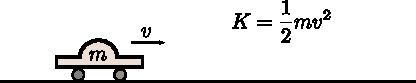
\includegraphics[scale = 1]{figures/hreyfiorka2.pdf}
    \caption{Hreyfiorka bíls með massa $m$ sem keyrir með hraðanum $v$.}
    \label{fig:hreyfiorka}
\end{subfigure}
\hfill
\begin{subfigure}[b]{.45\textwidth}
    \centering
    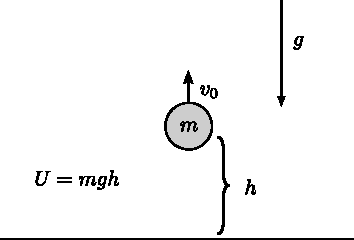
\includegraphics[scale = 1]{figures/stoduorkasimple.pdf}
    \caption{Stöðuorka bolta með massa $m$ sem er staddur í hæð $h$ í þyngdarsviði með þyngdarhröðun $g$.}
    \label{fig:stoduorkasimple}
\end{subfigure}
\caption{Myndræn skilgreining á hreyfiorku og stöðuorku.}
\end{figure}

\begin{tcolorbox}
\begin{theorem}
Lítum á hlut með massa $m$ í frjálsu falli í þyngdarsviði með þyngdarhröðun $g$. Gerum ráð fyrir að engin loftmótstaða verki á hlutinn. Látum $v$ tákna hraða hlutarins og látum $h$ tákna hæð hlutarins sem fall af tíma $t$. Þá er stærðin: 
\begin{align*}
    E = K + U = \frac{1}{2}mv^2 + mgh,
\end{align*}
varðveitt stærð sem nefnist \textbf{heildarorka} eða einfaldlega \textbf{orka} hlutarins.
\end{theorem}
\end{tcolorbox}

\textbf{Útleiðsla:} Við skulum hafa mynd \ref{fig:stoduorka} í huga í þessari útleiðslu. Segjum sem svo að upphafshraði hlutarins sé $v_0$ og að á þeim tíma sé hann staddur í hæð $h_0$. Við höfum þá samkvæmt tímaóháðu stöðujöfnunni að:
\begin{align*}
    -2g(h-h_0) = v^2 - {v_0}^2.
\end{align*}
En það þýðir einmitt að $v^2 = {v_0}^2 - 2g(h-h_0)$ svo við fáum:
\begin{align*}
    E = \frac{1}{2}mv^2 + mgh = \frac{1}{2}m\left( {v_0}^2 -2g(h-h_0) \right) + mgh = \frac{1}{2}m{v_0}^2 + mgh_0 = E_0.
\end{align*}
En það sýnir einmitt að, heildarorkan, $E = K + U$, er óháð tíma og því varðveitt. \qed

\begin{figure}[H]
    \centering
    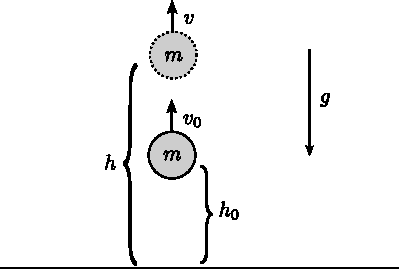
\includegraphics{figures/stoduorka.pdf}
    \caption{Hlutur með massa $m$ sem fer úr hæð $h_0$ í hæð $h$ í þyngdarsviði með þyngdarhröðun $g$.}
    \label{fig:stoduorka}
\end{figure}

Ef orkan er varðveitt í kerfinu sem við erum að skoða (hún er ekki endilega alltaf varðveitt í öllum þeim kerfum sem við skoðum) þá skrifum við einnig:
\begin{align*}
    E_{\text{fyrir}} = E_{\text{eftir}}.
\end{align*}

\newpage

\section{Árekstrar}

Til þess að tala um áreksta þá er gott að kynna til sögunnar hugtakið um skriðþunga:

\begin{tcolorbox}
\begin{definition}
Lítum á hlut með massa $m$ og hraða $v$. \textbf{Skriðþungi} hlutarins, $p$, er stærðin
\begin{align*}
    p = mv.
\end{align*}
\end{definition}
\end{tcolorbox}
Við tökum eftir því að einingar skriðþunga eru gefnar með $[
p] = [mv] = [m] \cdot [v] = \si{kg.m/s}$. Við tökum einnig eftir því að við höfum:
\begin{align*}
    K = \frac{1}{2}mv^2 = \frac{m^2 v^2}{2m} = \frac{p^2}{2m}.
\end{align*}

Með mynd \ref{fig:arekstur} í huga skulum við setja fram næsta varðveislulögmál:

\begin{tcolorbox}
\begin{theorem}
Lítum á tvo hluti, annan með massa $m_1$ og upphafshraða $v_1$, hinn með massa $m_2$ og upphafshraða $v_2$. Gerum ráð fyrir því að þeir lendi í árekstri við hvorn annann. Þá gildir:
\begin{align*}
    m_1 v_1 + m_2 v_2 = m_1 u_1 + m_2 u_2
\end{align*}
þar sem $u_1$ er hraði massans $m_1$ eftir áreksturinn og $u_2$ er hraði massans $m_2$ eftir áreksturinn.
\end{theorem}
\end{tcolorbox}

\textbf{Útleiðsla:} Við frestum formlegri útleiðslu þar til í kafla 6. Sannreyna má lögmálið með tilraun! \qed

\begin{figure}[H]
    \centering
\begin{subfigure}[h]{.4\textwidth}
    \centering
    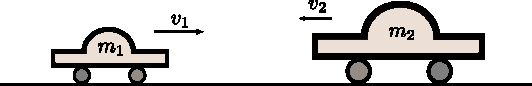
\includegraphics[width=\linewidth]{figures/farekstur.pdf}
    \caption{Fyrir áreksturinn}
    \label{fig:farekstur}
\end{subfigure}
\hfill
\begin{subfigure}[h]{.4\textwidth}
    \centering
    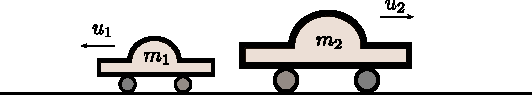
\includegraphics[width=\linewidth]{figures/earekstor.pdf}
    \caption{Eftir áreksturinn}
    \label{fig:earekstor}
\end{subfigure}
\caption{Árekstur tveggja bíla fyrir og eftir áreksturinn.}
\label{fig:arekstur}
\end{figure}

Ef skriðþunginn er varðveittur í kerfinu sem við erum að skoða (hann er ekki endilega alltaf varðveittur í öllum þeim kerfum sem við skoðum) þá skrifum við einnig:
\begin{align*}
    p_{\text{fyrir}} = p_{\text{eftir}}
\end{align*}

Undir venjulegum kringumstæðum glatast hluti af hreyfiorkunni í árekstrum í mismunandi þætti eins og til dæmis hljóð og varma. Þess vegna skoppar skopparabolti ekki eins hátt upp eftir hvert skopp. Við höfum hinsvegar eftirfarandi lögmál:

\begin{tcolorbox}
\begin{theorem}
Orkan, $W$, sem losnar í árekstri er jöfn breytingunni í hreyfiorku kerfisins,
\begin{align*}
    W = \Delta K = K_{\text{eftir}} - K_{\text{fyrir}}. 
\end{align*}
\end{theorem}
\end{tcolorbox}

\textbf{Útleiðsla:} Við frestum formlegri útleiðslu þar til í kafla 6.  \qed

\vspace{0.25cm}

Við viljum einnig hafa einhverja leið til þess að meta hversu skoppandi hlutir eru eða með öðrum orðum, hversu fjaðrandi.

\begin{tcolorbox}
\begin{definition}
Við segjum að árekstur tveggja eða fleiri hluta sé
\begin{enumerate}[label = \textbf{(\roman*)}]
    \item \textbf{alfjaðrandi} ef hreyfiorka kerfisins er varðveitt.
    \item \textbf{ófjaðrandi} ef hreyfiorka kerfisins er ekki varðveitt.
    \item \textbf{fullkomlega ófjaðrandi} ef hlutirnir festast saman eftir áreksturinn.
\end{enumerate}
\end{definition}
\end{tcolorbox}



\begin{tcolorbox}
\begin{theorem}
Lítum á tvo hluti, annan með massa $m_1$ og upphafshraða $v_1$, hinn með massa $m_2$ og upphafshraða $v_2$. Gerum ráð fyrir því að þeir lendi í alfjaðrandi árekstri. Þá gildir að:
\begin{align*}
    v_1 + u_1 = v_2 + u_2.
\end{align*}
\end{theorem}
\end{tcolorbox}

\textbf{Útleiðsla:} Við höfum samkvæmt skriðþungavarðveislu að:
\begin{align*}
    m_1 v_1 + m_2 v_2 = m_1 u_1 + m_2 u_2,
\end{align*}
og þar sem að áreksturinn er alfjaðrandi þá höfum við samkvæmt orkuvarðveislu að:
\begin{align*}
    \frac{1}{2}m_1 {v_{1}}^2 + \frac{1}{2}m_2 {v_{2}}^2 = \frac{1}{2}m_1 {u_{1}}^2 + \frac{1}{2}m_2 {u_{2}}^2.
\end{align*}
Nú kemur smá algebrutrikk, við athugum að við getum umritað orkujöfnuna sem:
\begin{align*}
    \frac{1}{2}m_1\left({v_1}^2 - {u_1}^2 \right) = \frac{1}{2}m_2 \left( {u_2}^2 - {v_2}^2 \right),
\end{align*}
og með því að nota samokaregluna sjáum við að:
\begin{align} \label{eq:arndis1}
    \frac{1}{2}m_1 \left( v_1 - u_1 \right)\left( v_1 + u_1 \right) = \frac{1}{2}m_2 \left( u_2 - v_2 \right) \left( u_2 + v_2 \right).
\end{align}
Við getum umritað skriðþungajöfnuna sem:
\begin{align} \label{eq:arndis2}
    m_1 \left( v_1 - u_1 \right) = m_2 \left( u_2 - v_2 \right)
\end{align}
Deilum núna jöfnu (\ref{eq:arndis1}) með jöfnu (\ref{eq:arndis2}) og styttum út tvistinn til að fá:
\begin{equation*}
    v_1 + u_1 = v_2 + u_2.
\end{equation*}
\qed

\vspace{0.2cm}

Þegar við tölum um árekstra þá getur verið þægilegt að gefa þeim tölu sem lýsir því hversu fjaðrandi þeir eru, við kynnum því:

\begin{tcolorbox}
\begin{definition}
Við skilgreinum \textbf{fjaðurstuðul} eða \textbf{skoppstuðull} áreksturs sem stærðina:
\begin{align*}
    \varepsilon := \frac{\text{afstæður hraði eftir árekstur}}{\text{afstæður hraði fyrir árekstur}} = \frac{u_1 - u_2}{v_1 - v_2}.
\end{align*}
\end{definition}
\end{tcolorbox}
Takið eftir að fjaðurstuðullinn er einingarlaus stærð. Yfirleitt gildir að $\varepsilon \in [0,1]$ því að hlutirnir glata hluta af hraða sínum í árekstrinum. Hinsvegar eru til efnasamsetningar þannig að $\varepsilon > 1$ en það er afar sjaldgæft.


\begin{figure}[H]
    \centering
    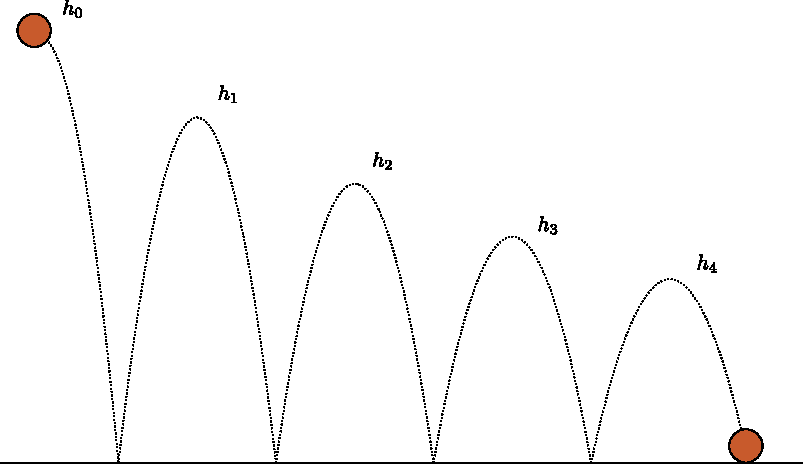
\includegraphics[scale = 0.8]{figures/skopparisimple.pdf}
    \caption{Skopparabolti missir hluta af hæð sinni vegna þess að skoppstuðullinn hans er lægri en $1$.}
    \label{fig:my_label}
\end{figure}


\newpage

\section{Dæmi}

\begin{enumerate}[label = \textbf{Dæmi \thechapter.\arabic*.}]

\subsection*{Orka}

\item Bíll með massann $m = \SI{650}{kg}$ keyrir með hraðanum $v = \SI{95}{km/klst}$.
\begin{enumerate}[label = \textbf{(\alph*)}]
    \item Hver er hreyfiorka bílsins?
    \item Hver er stöðuorka bílsins?
    \item Hver er heildarorka bílsins?
\end{enumerate}

\item Þröstur nokkur hefur massa $\SI{35}{g}$ og flýgur með hraðanum $\SI{45}{km/klst}$ í $\SI{4.8}{m}$ hæð.
\begin{enumerate}[label = \textbf{(\alph*)}]
    \item Hver er hreyfiorka þrastarins?
    \item Hver er stöðuorka þrastarins? 
    \item Hver er heildarorka þrastarins?
\end{enumerate}

\item Lítum á bolta með massa $m = \SI{0.58}{kg}$ sem er sleppt úr kyrrstöðu í upphafshæð $h_0 = \SI{14.3}{m}$.
\begin{enumerate}[label = \textbf{(\alph*)}]
    \item Hver er stöðuorka boltans áður en honum er sleppt?
    \item Hver er heildarorka boltans?
    \item Hver er hreyfiorka boltans þegar hann hefur fallið niður í hæð $h = \SI{7.3}{m}$?
    \item Hver er hraði boltans þegar hann er í hæðinni $h = \SI{7.3}{m}$?
\end{enumerate}

\item Lítum á mynd \ref{fig:sbrkassar} hér að neðan. Hvaða kassi er með mesta hreyfiorku?

\begin{figure}[H]
    \centering
    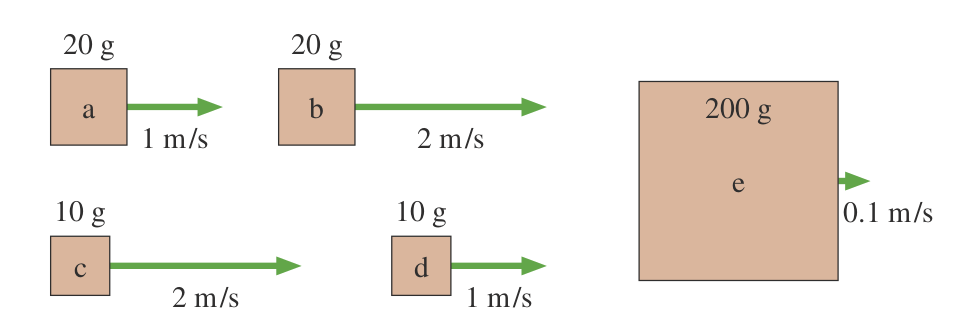
\includegraphics[scale = 0.3]{images/sbr.png}
    \caption{Nokkrir kassar.}
    \label{fig:sbrkassar}
\end{figure}

\item Hjálmtýr hjólreiðamaður er $\SI{90}{kg}$. Hann hjólar á jafnsléttu með hraða $\SI{6.0}{km/klst}$ en gefur síðan í og nær hraðanum $\SI{12}{km/klst}$. Hversu mikil breyting varð í hreyfiorku Hjálmtýs. Hvaðan kom þessi orka?

\item Við stofuhita er hreyfiorka súrefnissameindar, $O_2$, gefin með $ K = \SI{6.21e-21}{J}$. Massi einnar róteindar er $m_r = \SI{1.67e-27}{kg}$. Metið hraða súrefnissameindarinnar.

\item Kárahnjúkavirkjun er $\SI{193}{m}$ á hæð. Þar rennur Jökulsá á Fjöllum framaf. Meðalrennsli Jökulsár er \SI{110}{m^3/s}. Metið orkuna sem hægt er að virkja á einu ári.

\item Skíðakappi nokkur rennir sér niður Töfrateppið í Bláfjöllum. Brekkan hallar um \ang{12} miðað við lárétt. Brekkan byrjar í $\SI{105}{m}$ hæð. Hver verður hraði skíðakappans þegar hann kemur niður brekkunna ef svo gott sem enginn núningur verkar á skíðin hans? Hvað ef hornið hefði verið \ang{25}?

\item Sleða er ýtt upp brekku sem hallar um \ang{22.5} miðað við lárétt með upphafshraða $v = \SI{7.2}{m/s}$. Sleðinn nær mestri hæð $h$ áður en hann byrjar að renna aftur niður. Gerum ráð fyrir að enginn núningur verki á sleðann. Hversu hátt kemst sleðinn? Hver er hraði sleðans þegar hann er búinn að renna aftur niður?

\subsection*{Skriðþungi}

\item Bíll með massann $m = \SI{650}{kg}$ keyrir með hraðanum $v = \SI{95}{km/klst}$. Hver er skriðþungi bílsins?

\item Þröstur nokkur hefur massa $\SI{35}{g}$ og flýgur með hraðanum $\SI{45}{km/klst}$. Hver er skriðþungi þrastarins?

\item Lítum á mynd \ref{fig:sbrkassar2} hér að neðan. Hvaða kassi er með mestan skriðþunga?

\begin{figure}[H]
    \centering
    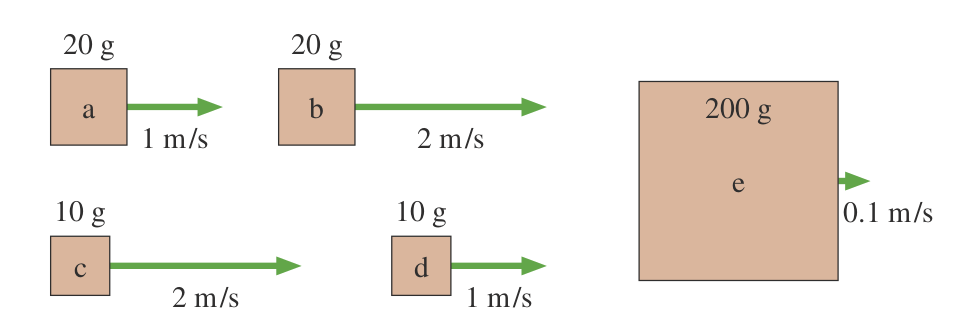
\includegraphics[scale = 0.3]{images/sbr.png}
    \caption{Nokkrir kassar.}
    \label{fig:sbrkassar2}
\end{figure}

\begin{minipage}{\linewidth}

\begin{wrapfigure}{r}{2.1in}
\centering
\vspace{-1cm}
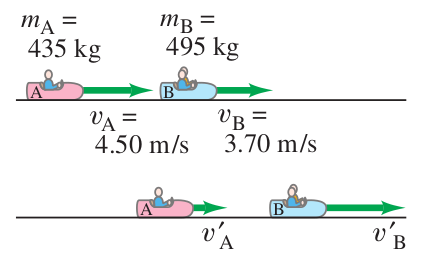
\includegraphics[width=2.1in]{images/bumber.png}
    \label{fig:bumper}
\end{wrapfigure}

\item Tveir klessubílar lenda í alfjaðrandi árekstri í Skemmtigarðinum í Smáralind. Amelía klessir aftan á Berg. Heildarmassinn á klessubíl Amelíu (ásamt henni) er $m_A = \SI{435}{kg}$ og heildarmassinn á klessubíl Bergs er $m_B = \SI{455}{kg}$. Hraði Amelíu fyrir áreksturinn er $v_A = \SI{4.50}{m/s}$ og hraði Bergs fyrir áreksturinn er $v_B = \SI{3.70}{m/s}$. Hver verður hraði þeirra eftir árksturinn? 
\end{minipage}

\item Friðbert stekkur um borð í kyrrstæðan fleka í vatni á hraðanum $\SI{5.0}{m/s}$. Massi Friðberts er $\SI{50}{kg}$ en massi flekans er $\SI{200}{kg}$. Hver verður hraði flekans þegar Friðbert er lentur á honum?

\item Þanos stendur í vagni sem rennur með hraðanum $v_0 = \SI{16.0}{m/s}$ eftir núningslausum fleti. Í vagninum eru sex stórir steinar, hver með massann $m_{s}=\SI{88}{kg}$. Vagninn hefur massann $m_{v}=\SI{800}{kg}$ og massi Þanosar er $m_{\text{Þ}}=\SI{445}{kg}$.
\begin{enumerate}[label = \textbf{(\alph*)}]
    \item Hver er skriðþungi vagnsins ásamt innihaldi?
    \item Captain Marvel er að reyna ná Þanosi og þeytist að honum með hraðanum $v_{M}= \SI{200}{m/s}$. Þanosi dettur það snilldarráð í hug að kasta steinum frá borði til þess að auka hraðann sinn. Hvað þarf Þanos að kasta hverjum stein með miklum hraða til þess að ná hraðanum $\SI{200}{m/s}$ og koma í veg fyrir að Captain Marvel nái honum og berji hann í spað?
\end{enumerate}

\item Járnbrautalest með massa $\SI{5000}{kg}$ rennur meðfram núninglausum járnbrautateinum með hraða $\SI{22}{m/s}$. Skyndilega byrjar að rigna og lestin byrja að fyllast af vatni. Nokkrum mínútum síðar hefur aukna þyngd vatnsins hægt á lestinni þannig að hraði hennar er $\SI{20}{m/s}$. Hver er massi vatnsins?

\vspace{0.3cm}

\begin{minipage}{\linewidth}
\begin{wrapfigure}{r}{1.9in}
\centering
\vspace{-0.5cm}
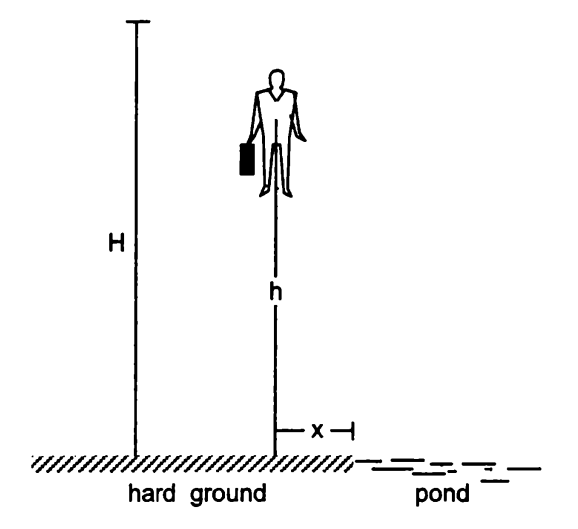
\includegraphics[width=2.6in]{images/pond.png}
   \label{fig:amypond}
\end{wrapfigure}

\item Lalli lögfræðingur hefur massa $M = \SI{87}{kg}$ og heldur á skjalatösku með massa $m = \SI{7.2}{kg}$. Hann fellur óvart framaf skrifstofubygginginni sinni úr hæð $H = \SI{95}{m}$. Sekúndu síðar, þegar hann er staddur í hæð $h = \SI{90}{m}$ áttar hann sig á því að fyrir neðan hann er hart malbik en í lóðréttri fjarlægð $x = \SI{1.5}{m}$ er tjörn sem gæti bjargað lífi hans. Hann nýtir sér því skriðþungavarðveislu og hendir því skjalatöskunni sinni með hraða $v$ 
frá tjörninni. Finnið minnsta hraða $v$ sem að hann getur kastað töskunni þannig að hann lifi af fallið. Hvar lendir taskan?

\end{minipage}

\newpage



\begin{minipage}{\linewidth}
\begin{wrapfigure}{r}{1.9in}
\centering
\vspace{-1cm}
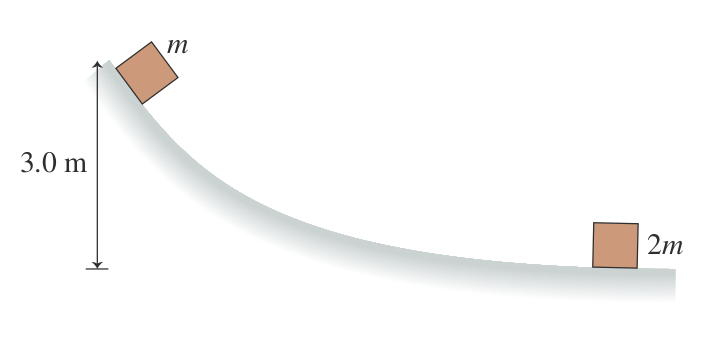
\includegraphics[width=2.6in]{images/skab.png}
   \label{fig:vifilfell}
\end{wrapfigure}

\subsection*{Varðveislulögmálin}

\item Kristinn kærulausi er að vinna lagerstarf hjá Ölgerðinni. Hann er með kassa með massa $m = \SI{6.0}{kg}$ sem hann lætur renna niður núningslausa braut úr $\SI{3.0}{m}$ hæð. Við enda brautarinnar sendur kassi sem hefur massa $2m = \SI{12.0}{kg}$.

\end{minipage}

\begin{enumerate}[label = \textbf{(\alph*)}]
    \item Gerum ráð fyrir að kassarnir festist saman eftir áreksturinn, þ.e.~að þeir lendi í fullkomlega ófjaðrandi áresktri. Hver verður hraði kassanna eftir áreksturinn?
    \item Gerum nú ráð fyrir að kassarnir lendi í fullkomlega fjaðrandi árekstri. Í hvaða hæð kemst kassinn með massa $m$ þegar hann fer aftur upp brautina?
\end{enumerate}

\item Tvær járnbrautalestir, báðar með massa $m = \SI{66000}{kg}$ og hraða $v = \SI{120}{km/klst}$ lenda í árekstri. Hversu mikil orka losnar við áreksturinn? Hvert fór orkan?

\item Kúlu $A$ er skotið með hraða $\SI{4.0}{m/s}$ á kúlu $B$ sem er kyrr. Þegar $A$ klessir á $B$ endurkastast $A$ með hraða $\SI{0,5}{m/s}$ í sömu stefnu og hún kom úr. Hvaða hraða fær $B$ ef áreksturinn er alfjaðrandi?

\vspace{0.5cm}


\begin{minipage}{\linewidth}
\begin{wrapfigure}{r}{1.8in}
\centering
\vspace{-0.5cm}
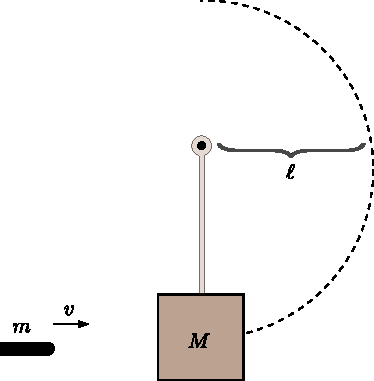
\includegraphics[width=2.3in]{figures/pendullkula2.pdf}
   \label{fig:pendulkula}
\end{wrapfigure}

\item Bolta er sleppt úr upphafshæð $h_0 = \SI{1.60}{m}$ og skoppar aftur upp í hæð $h_1 = \SI{1.20}{m}$ eftir fyrsta skopp. Hver er skoppstuðull boltans? Hversu oft mun boltinn þurfa að skoppa þar til að hæðin sem boltinn nær eftir skopið verður orðin lægri en $\SI{0.1}{m}$?

\item Pendúll samanstendur af kubb með massa $M = \SI{672}{g}$ sem hangir í massalausum vír af lengd $\ell = \SI{0.32}{m}$. Nú er byssukúlu með massa $m = \SI{3.56}{g}$ og hraða $v$ skotið inn í kubbinn þannig að kúlan festist inni í honum. Hvert er minnsta gildið á hraðanum $v$ þannig að pendúllinn nái að sveiflast framhjá hæstu stöðu?


\item Loftsteinn með massa $m_\ell = \SI{4.6e15}{kg}$ lendir í árekstri við jörðina (sem hefur massa $M_J = \SI{5.94e24}{kg}$). Hraði loftsteinsins fyrir áreksturinn var $v_\ell = \SI{25}{km/s}$ (afstætt miðað við viðmiðunarkerfi þar sem jörðin er kyrr) og áreksturinn er fullkomlega ófjaðrandi (loftsteinninn staðnæmist á yfirborði jarðarinnar).

\end{minipage}

\begin{enumerate}[label = \textbf{(\alph*)}]
    \item Með hversu miklum hraða endurkastaðist jörðin eftir áreksturinn?
    
    \item Reiknið orkuna sem losnaði við áreksturinn, $\Delta K = K_{\text{eftir}} - K_{\text{fyrir}}$.
    
    \item Til samanburðar er orkan sem losnar í kjarnorkusprengju um það bil $\SI{4.0e16}{J}$. Hversu margar slíkar sprengjur þyrfti að sprengja á sama tíma til þess að jafnast á við eyðileggingarmátt loftsteinsins? 
\end{enumerate}

\item Kubbur með massa $\SI{50}{kg}$ ferðast með hraða $\SI{20}{km/klst}$. Hann lendir í árekstri við annan kubb með massa $\SI{20}{kg}$ sem ferðast í gagnstæða stefnu með hraða $-\SI{10}{km/klst}$. Kubbarnir festast saman eftir áreksturinn. Hver er hraði kubbanna eftir áreksturinn? Hver er skoppstuðull kubbanna?

\item Kassi með massa $m = \SI{1.5}{kg}$ ferðast með hraða $v = \SI{2.2}{m/s}$ og rekst á annan kyrrstæðan kassa með massa $2m = \SI{3.0}{kg}$. Léttari kassinn staðnæmist eftir áreksturinn. Hver er skoppstuðull kassanna?

\item Kassi með massa $M$ og hraða $V$ lendir í alfjaðrandi árekstri við kyrrstæðan kassa með massa $m$. Látum $V_M$ og $v_m$ tákna hraða annarsvegar $M$ og hinsvegar $m$ eftir áreksturinn. Sýnið að:
\begin{align*}
    V_M = \frac{(M-m)V}{M+m}, \hspace{0.8cm} v_m = \frac{2MV}{M + m}
\end{align*}

\item Sýnið að árekstur sé alfjaðrandi þá og því að eins að hann hafi fjaðurstuðul $\varepsilon = 1$.

\newpage

\subsection*{Erfið dæmi}

\begin{minipage}{\linewidth}
\begin{wrapfigure}{r}{1.5in}
\centering
\vspace{-1cm}
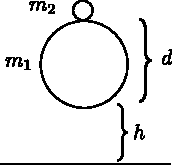
\includegraphics{figures/highflying.pdf}
   \label{fig:ipho1966}
\end{wrapfigure}

\item \textbf{(Eðlisfræðikeppni framhaldsskólanna 2012)} Tennisbolti með massa $m_2$ situr á körfubolta með massa $m_1$. Neðsti hluti körfuboltans er í hæð $h$ en neðsti hluti tennisboltans er í hæð $h + d$. Boltunum er sleppt samtímis. Þegar tennisboltinn skoppar aftur upp kemst neðsti hluti hans hæst í hæð $H$. Gerum ráð fyrir að $m_1 \gg m_2$, að allir árekstrarnir séu alfjaðrandi og að hunsa megi loftmótstöðu. Ákvarðið hæðina $H$ sem fall af $h$ og $d$.
\end{minipage}

\vspace{0.5cm}

\item \textbf{(\href{https://youtu.be/HEfHFsfGXjs}{3blue1brown})} Lítum á tvo kassa með massa, $m$ og $M$ eins og á mynd \ref{fig:3blue1brown}. Látum upphafshraða massa $M$ vera $v_0$ til vinstri. Gerum ráð fyrir að enginn núningur verki á kassana og að allir árekstrarnir sem þeir lenda í séu alfjaðrandi árekstrar.

\begin{enumerate}[label = \textbf{(\alph*)}]
    \item Skoðum tilvikið þegar að massarnir hafa sama massa, $M = m = \SI{1}{kg}$. Til einföldunar látum við $v_0 = \SI{1}{m/s}$. Hversu margir árekstrar verða ef við teljum líka með árekstra við vegginn?
    
    \item Skoðum tilvikið þegar $v_0 = \SI{1}{m/s}$, $m = \SI{1}{kg}$ en $M = \SI{10}{kg}$. Hversu margir árekstrar verða þá?
    
    \item Reyndar er fjöldi árekstra óháður upphafshraðanum $v_0$. Heildarfjöldi árekstranna verður:
    \begin{align*}
        N \approx \pi \sqrt{\frac{M}{m}}.
    \end{align*}
    Látum nú $m = \SI{1}{kg}$ og $M = 10^{2d} \, \si{kg}$ þar sem $d \in \N$. Hver verður heildarfjöldi árekstra þá?
\end{enumerate}


\begin{figure}[H]
    \centering
    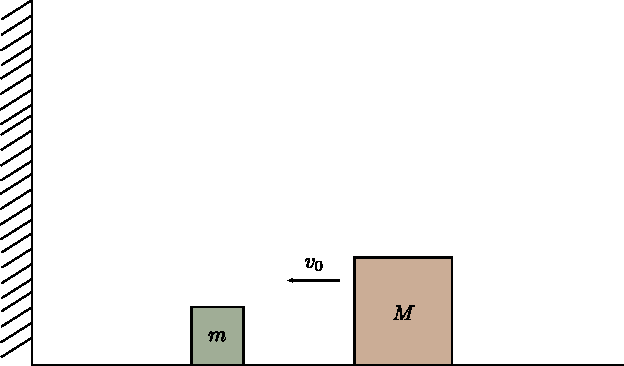
\includegraphics[scale = 0.8]{figures/3b1b.pdf}
    \caption{Kassarnir tveir í 3blue1brown dæminu.}
    \label{fig:3blue1brown}
\end{figure}

\begin{minipage}{\linewidth}
\begin{wrapfigure}{r}{3.5in}
\centering
\vspace{-0.5cm}
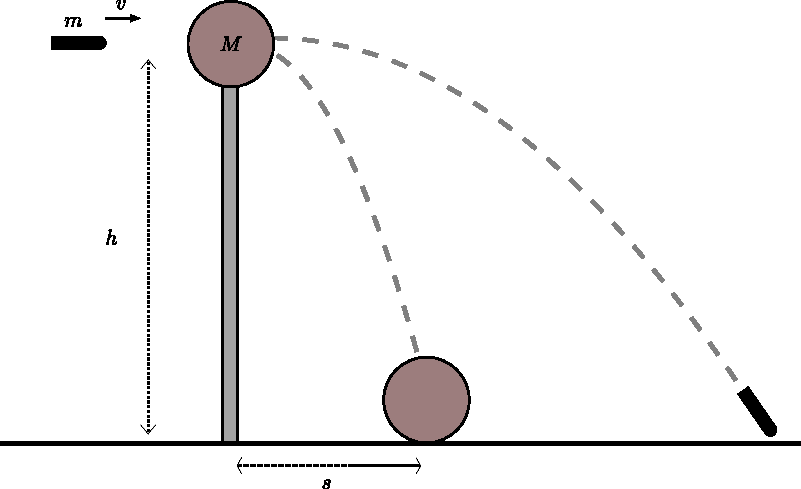
\includegraphics[scale = 0.8]{figures/ipho1966.pdf}
   \label{fig:ipho1966}
\end{wrapfigure}

\item \textbf{(IPhO, 1967)} Lítill bolti með massa $M = \SI{0.2}{kg}$ hvílir ofan á lóðréttri súlu í hæð $h = \SI{5}{m}$. Byssukúlu með upphafshraða $v_0 = \SI{500}{m/s}$ og massa $m = \SI{0.01}{kg}$ er skotið í átt að boltanum. Byssukúlan fer lárétt í gegnum miðju kúlunnar. Boltinn lendir í láréttri fjarlægð, $s = \SI{20}{m}$, frá súlunni. Hvar lendir byssukúlan? Hversu stórt hlutfall af hreyfiorku byssukúlunnar breyttist í varma þegar hún fór í gegnum boltann? Hunsið loftmótstöðu.  

\end{minipage}

\end{enumerate}

\newpage